\let\negmpace\undefined
\let\negthickspace\undefined
\documentclass[journal]{IEEEtran}
\usepackage[a5paper, margin=10mm, onecolumn]{geometry}
%\usepackage{lmodern} % Ensure lmodern is loaded for pdflatex
% Include tfrupee package
\setlength{\headheight}{1cm} % Set the height of the header box
\setlength{\headsep}{0mm}     % Set the distance between the header box and the top of the text
\usepackage{xparse}
\usepackage{gvv-book}
\usepackage{gvv}
\usepackage{cite}

\usepackage{amsmath,amssymb,amsfonts,amsthm}
\usepackage{algorithmic}
\usepackage{graphicx}
\usepackage{textcomp}
\usepackage{xcolor}
\usepackage{txfonts}
\usepackage{listings}
\usepackage{enumitem}
\usepackage{mathtools}
\usepackage{gensymb}
\usepackage{comment}
\usepackage[breaklinks=true]{hyperref}
\usepackage{tkz-euclide} 
\usepackage{listings}
% \usepackage{gvv}                                        
\def\inputGnumericTable{}                                 
\usepackage[latin1]{inputenc}                                
\usepackage{color}                                            
\usepackage{array}                                            
\usepackage{longtable}                                       
\usepackage{calc}                                             
\usepackage{multirow}                                         
\usepackage{hhline}                                           
\usepackage{ifthen}                                           
\usepackage{lscape}
\renewcommand{\thefigure}{\theenumi}
\renewcommand{\thetable}{\theenumi}
\setlength{\intextsep}{10pt} % Space between text and floats
\numberwithin{equation}{enumi}
\numberwithin{figure}{enumi}
\renewcommand{\thetable}{\theenumi}
\begin{document}
\bibliographystyle{IEEEtran}
\title{9.4.4}
\author{EE24BTECH11033 - KOLLURU SURAJ}
% \maketitle
% \newpage
% \bigskip
{\let\newpage\relax\maketitle}
\textbf{Question:} 
$x\frac{dy}{dx}-y=2x^2$
\\\\
\solution\\
Divide the given equation with $x$
\begin{align}
    \frac{dy}{dx}-\frac{y}{x}=2x\label{1} 
\end{align}
Which is a linear differential equation of the type $\frac{dy}{dx} +Py=Q$\\ where
\begin{align}
P= -\frac{1}{x}\\
Q=2x
\end{align}

$\text{I.F.} = e^{\int -\frac{1}{x} \, dx} = e^{-\log x} = e^{\log \frac{1}{x}} = \frac{1}{x} \quad \text{[as } e^{\log f(x)} = f(x) \text{]}$\\

Hence, the Integrating factor is $\frac{1}{x}$\\
Therefore, solution of the given equation is given by\\
\begin{align}
    \frac{y}{x}=\int 2dx\\
    \frac{y}{x}=2x+c\\
    y=2x^2+cx
\end{align}
Take initial condition as x= 1, y= 1. We get c= -1
\begin{align}
    y=2x^2- x
\end{align}


\noindent\textbf{Numerical Approach:}\\1. I used a for loop for finding the $y$ values as the loop proceeds with iterative formula given below. I took some initial value of $x$ and as loop proceeds I assigned it the value as $x+h$. where $h$ is the step size, representing the rate of change. 
\\2. Assigned the values of $y$ for different $x$-values using a for loop. \\ 
3. Here the initial value of x is 1 and y is 1\\
\\ \textbf{Using the Method of Finite Differences}\\
The Method of Finite Differences is a numerical technique used to approximate solutions to differential equations. 

We know that:
\begin{align}
   \lim_{h \to 0} \frac{y(x+h) - y(x)}{h} &= \frac{dy}{dx} 
\end{align}
For the given differential equation \ref{1},
\begin{align}
    \frac{dy}{dx}&= \frac{y}{x}+2x\\
    \frac{y_{n+1} - y_n}{h}&\approx \frac{y_n}{x_n}+2x_n\\
    y_{n+1} &= y_n + \brak{\frac{y_n}{x_n}+2x_n}\cdot h
\end{align}
The iterative formula for updating $x$-values is: 
\begin{align}
    x_n=x_{n-1}+h
\end{align}
Using Matplotlib, I plotted the computed points and the graph of the exact solution to verify that they approximately match
\begin{figure}[!ht]
    \centering
    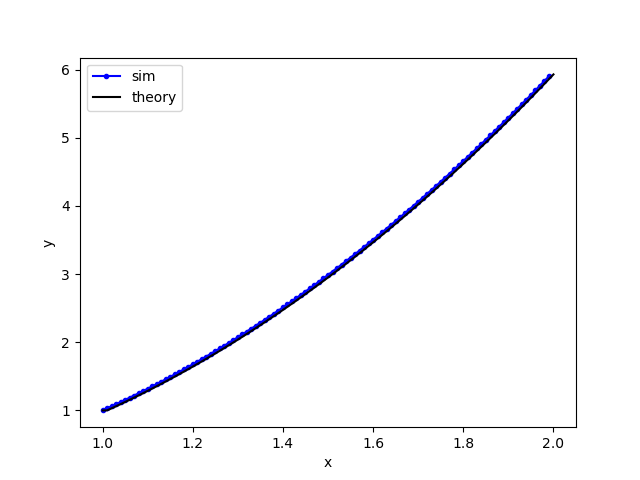
\includegraphics[width=\columnwidth]{figs/Figure_1.png}
    \caption{}
\end{figure}


\end{document}
